\subsection{Plataforma \jason} \label{sec:aoppj}

A presente seção visa explicar a plataforma \jason baseada na arquitetura BDI.
Essa arquitetura é baseada no que o agente sabe ou guarda (crenças), as opções
que ele possui de atuação baseado em suas próprias regras (desejos) e seus
comprometimentos (intenções). Assim, na seção \ref{sec-jason-overview} uma
visão geral da plataforma é apresentada e em seguida a engenharia da mesma é
discutida.

\subsubsection{Visão Geral} \label{sec-jason-overview}

Para uma explicação mais didática será utilizado o exemplo \emph{Room} que
acompanha o \emph{Jason}. Para isso será introduzido
o arquivo de projeto do exemplo e, a partir desse, os demais arquivos.
A Listagem~\ref{lst-roomMas2j} contém o arquivo de projeto.
Na linha 2 da listagem, \emph{room} é o nome do projeto e, por isso, pode ser qualquer
identificador. A partir da linha 3 os valores antes dos dois-pontos (:)
são palavras reservadas que o \jason entende para diferentes propósitos e o valor
a seguir (depois dos dois-pontos) é o valor associado.
Assim, \emph{infrastructure}, na linha 3, pode assumir três valores
possíveis: (i) \emph{Centralised}, normalmente utilizada;
(ii) \emph{Jade}, utilizada quando se deseja integrar
com agentes não \jason (jade) ou rodar distribuído na rede; (iii) \emph{Saci}, utilizada
quando deseja executar os agentes de maneira distribuída na rede.

\begin{center}
    \begin{minipage}{120mm}
	\lstset{linewidth=120mm}
	\begin{lstlisting}[frame=trbl, caption=Arquivo de projeto do \jason para o exemplo \emph{Room}, label=lst-roomMas2j]
// Isso eh um comentario
MAS room {
  infrastructure: Centralised
  environment: RoomEnv
  executionControl: jason.control.ExecutionControl
  agents: porter; claustrophobe; paranoid;
}
	\end{lstlisting}
    \end{minipage}
\end{center}

Continuando na Listagem~\ref{lst-roomMas2j}, a entrada \emph{environment}
configura a classe de ambiente que será utilizada. A próxima entrada,
normalmente não aparece, é a \emph{executionControl} utilizada para
mudar a forma com que os agentes são executados. O valor no exemplo é uma
classe que obriga o próximo ciclo de deliberação somente acontecer quando
todos os agentes terminaram o seu ciclo. O padrão é iniciar um novo
após 500ms do anterior ter sido concluído, porém, algumas vezes isso
pode vir a apresentar problemas de sincronismo por ser assíncrono e, por isso, é interessante
mostrar que há uma opção para controlar a forma de execução dos ciclos
deliberativos. O usuário, inclusive, pode colocar sua própria classe como
configuração.

Todas as entradas apresentadas até agora mapeiam para código Java.
Os agentes são especificados na entrada \emph{agents}. Como pode-se
observar na Listagem~\ref{lst-roomMas2j}, cada referência a um agente deve
terminar com um ponto-e-vírgula (;). Há ainda como especializar cada um dos
agentes mudando opções. Na seção~\ref{sec-jason-architecture} e no
capítulo~\ref{ch:cdu} são mostrados exemplos dessas opções.

Os agentes são desenvolvidos em arquivos texto com extensão \emph{ASL}, porém
antes de entrar em discussão sobre os agentes será explicado o exemplo sendo
utilizado. Nesse cenário tem-se uma porta na sala e duas pessoas, uma
claustrofóbica e outra paranoica. A pessoa claustrofóbica deseja que a
porta da sala esteja aberta, enquanto que a paranoica deseja que a porta
fique fechada.

Logo, há três agentes na linha 6 da Listagem~\ref{lst-roomMas2j}:
(i) \emph{porter}, o agente responsável pela porta e o único que conhece
como abri-lá ou fecha-lá;
(ii) \emph{claustrophobe}, o agente que deseja deixar a porta sempre aberta;
(iii) \emph{paranoid}, o agente que deseja deixar a porta sempre fechada.
A implementação desses agentes faz uso de eventos.

Esses eventos podem ser de adição (+) ou de remoção (-) de crenças, metas ou
consultas. Todas as estruturas são semelhantes a chamada de função. No
exemplo ``telefone(808080822)'', telefone pode ser uma crença ou uma ação de
ambiente que pode ser executada dependendo de onde a expressão aparece.
Note que, se essa entrada for precedida pelo sinal de exclamação (!) ou de
interrogação (?) então o significado é alterado para uma meta ou para uma
consulta respectivamente. Ainda há a possibilidade de preceder uma crença ou
meta com sinal de adição ou de subtração significando ou estar
adicionando/removendo uma crença ou estar adicionando/removendo uma meta ou
consulta.

\lstset{linewidth=75mm}
\begin{wrapfigure}{l}{85mm}
	\begin{lstlisting}[frame=trbl, caption=Agentes em ASL, label=lst-agente]
// claustrophobe.asl
+locked(door) : true
  <- .send(porter,achieve,~locked(door)).

// paranoid.asl
+~locked(door)
  <- .send(porter,achieve,locked(door)).

// porter.asl
+!locked(door)[source(paranoid)]
  : ~locked(door)
  <- lock.

+!~locked(door)[source(claustrophobe)]
  : locked(door)
  <- unlock.
	\end{lstlisting}
\end{wrapfigure}
%
Na Listagem~\ref{lst-agente} tem-se a continuação do exemplo e, por
simplicidade, todos os fontes dos agentes encontram-se reunidos. O agente denominado
\emph{claustrophobe} será o primeiro a ser detalhado e corresponde as linhas 1 até 3
da Listagem~\ref{lst-agente}. A programação em \jason é
guiada por reatividade às crenças e percepções do próprio agente, assim, é necessário
uma forma de estruturar as ações à serem decididas. Essa forma é o plano.
O plano pode ser ativado quando se deseja adicionar, consultar ou remover
\footnote{Uma remoção pode ser gerada devido a uma falha, porém isso não será
abordado.} uma crença ou meta. O plano da linha 2 até 3 da
Listagem~\ref{lst-agente} será detalhado adiante.

Em um plano há sempre três divisões: evento disparador, contexto e corpo.
A primeira e única à ser explicita é o evento disparador, que deve ocorrer para
o plano ser disparado. Ele está limitado do carácter inicial até
o dois-pontos (:). A divisão de contexto é onde se coloca as ações, crenças
ou regras que tem que ser válidas para o corpo do plano ser
considerado válido. Dessa forma, é
importante tomar cuidado no que vai no contexto em razão dele sempre ser
executado previamente para definir quais planos devem ser descartados da lista
de opções.
A segunda divisão vai até a seta (<-) e não é obrigatória.
A terceira divisão, também não é obrigatória, possui todas as ações a serem
executadas quando o plano tornar-se ativo.

No exemplo o plano tem em seu corpo
uma ação interna do \jason denominada \emph{send} que envia determinada
mensagem
(terceiro parâmetro) para o agente especificado (primeiro parâmetro) com
determinado propósito (segundo parâmetro). Uma ação interna possui o seguinte
formato ``tcp.send'', assim essa ação está definida no pacote \emph{tcp} pela
classe \emph{send} que deve especializar a classe \emph{DefaultInternalAction}
do \emph{Jason}. Entretanto, uma ação interna definida pelo \jason não possui
indicativo de pacote que é o caso do ``.send'' presente no código dos agentes.

No exemplo da linha 3 na Listagem~\ref{lst-agente}, o agente
\emph{claustrophobe} está enviando uma mensagem para o agente denominado
\emph{porter} ter a meta (\emph{achieve} no segundo parâmetro) de ter a crença
que a porta não ($\sim$) está fechada. Analogamente, o agente denominado
\emph{paranoid}, definido na linha 5 à 7, envia como crença ter a porta
fechada. Logo, o agente \emph{porter} pode ser entendido em sua quase
totalidade na Listagem~\ref{lst-agente}. Um entendimento completo do exemplo
vem com a compreensão das anotações que são informações que podem ser
guardadas junto das crenças e essas anotações podem ter suas próprias
anotações também. No agente \emph{porter} essas anotações são utilizadas
somente para dizer que determinado plano só é válido quando tiver como fonte
(do inglês \emph{source}) um determinado agente. O presente exemplo assume a
hipótese do mundo aberto. Vale observar que essas anotações podem ser
removidas sem nenhum problema adicional, entretanto, se isso for feito
assume-se a hipótese do mundo fechado e não seria possível ter um novo agente
que o \emph{porter} ignora.

A execução dos agentes acontece de forma arbitrária e deve-se ter em conta
que o primeiro agente que irá enviar a mensagem para o agente \emph{porter} dependerá
de como o mundo inicia. Logo, se o mundo iniciar com a porta fechada o primeiro
a enviar a solicitação será o agente \emph{claustrophobe}. Já se o mundo for iniciado
com a porta aberta o primeiro a enviar solicitação será o agente \emph{paranoid}.
Depois disso, conforme a simulação vai correndo, os dois agentes ficam alternando
mensagens com o agente \emph{porter} por causa do compartilhamento do mesmo
recurso (a porta).

\vfill

\subsubsection{Infra-estrutura do \jason} \label{sec-jason-architecture}

A plataforma \jason tem uma base de software completamente extensível como
é possível observar mediante a Figura \ref{fig-jason-infra-1}.
Nessa figura, a infra-estrutura encontra-se representada como um barramento
na parte inferior. Ela pode ser configurada através da chave de configuração
\emph{infrastructure} no arquivo de projeto (ver Listagem~\ref{lst-roomMas2j}).

A infraestrutura define todas as classes padrões que o usuário irá utilizar,
por exemplo observe que o barramento liga-se a dois adaptadores: um do tipo
agente e um de ambiente. Esses adaptadores permitem a compatibilidade entre
implementações distintas permitindo que ocorram variações sem ter que alterar
a estrutura do barramento.

\begin{figure}
               \begin{center}
               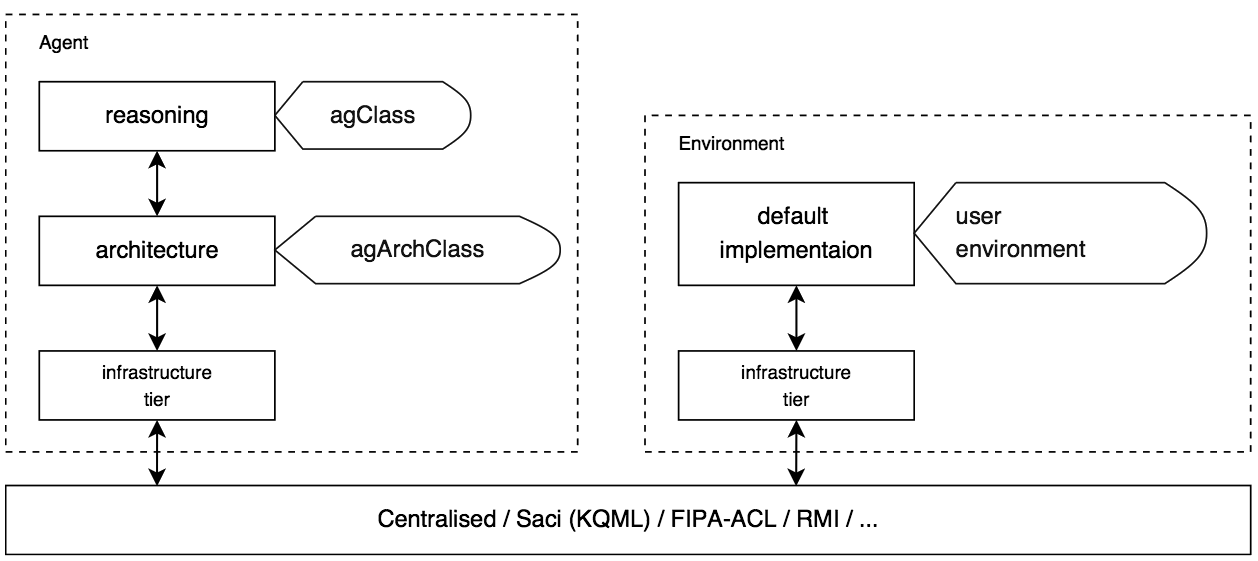
\includegraphics[width=140mm]{figuras/infra.png} 
                \end{center}
                \caption{Modelo da infra-estrutura do \emph{Jason}.}
                \label{fig-jason-infra-1}
\end{figure}

Assim, há a possibilidade de informar para uma determinada simulação que um
determinado agente utilizará uma arquitetura e/ou um raciocinador diferente
dos demais agentes. Para se fazer isso no momento que se declara os agentes
no projeto informa-se as chaves que encontram-se dentro das caixas com
cantos arqueados na Figura~\ref{fig-jason-infra-1}. O exemplo
``fb agArchClass KosMos.FireBrigadeArch agClass KosMos.Agent \#1;'' define
um (\#1) agente \emph{fb} com a arquitetura usando a classe \emph{FireBrigadeArch}
do pacote \emph{KosMos} (pode ser qualquer nome desejado) e configurando o
raciocinador a partir da classe \emph{Agent} do mesmo pacote. Note que, essas classes
não existem no \jason e devem ser providas pelo usuário de alguma forma.

Como já explicado, a entrada \emph{environment} no arquivo de projeto
configura a classe de ambiente que será utilizada e somente um
é permitido por simulação. Um dos motivos comuns de se implementar um
ambiente é implementar as ações que o agente poderá realizar no mesmo. Aliás,
também, é possível alterar como os agentes percebem o meio para, por
exemplo, inserir percepções incorretas em alguns momentos.

Essa infraestrutura extensível permitiu a implementação do trabalho de
\citet{moreira2006agent} por \citet{KlaBor09} sem nenhuma alteração profunda
nas classes da plataforma. Esse trabalho permitiu que o \jason usa-se
ontologias, inclusive definindo conceitos e compartilhando o conhecimento. Por
exemplo, um agente pode dizer para outro que a informação que ele deseja
encontra-se em determinada ontologia. Além disso, há outras extensões como
não usar arquivos de projeto e sim uma base de conhecimento baseada em
ontologia para definir a simulação.

O presente trabalho segue uma ideia parecida desses dois anteriores. A
principal preocupação era ter as crenças que a ontologia considere relevantes
em sua base de conhecimento e as outras guardadas na base padrão. Isso não é
diferente no trabalho anterior, o que é diferente é o como a relevância é
verificada. No trabalho anterior, o que era salvo na base era tudo que estivesse com a
anotação usada para indicar a ontologia e no presente desenvolvimento isso é
extraído da própria. Assim, se na ontologia contiver
o conceito Pizza e inserimos uma crença ``pizza(p1)''. O mecanismo
desenvolvido sabe que essa crença é relevante para a ontologia. Já o do
trabalho anterior para saber que o mesmo é relevante precisa ser marcado
com uma anotação, por exemplo ``pizza(p1)[ontology(URL)]''. Além disso, ele
não lida emoções e no presente trabalho os agentes podem perceberem seus
sentimentos.

